% !TeX program = xelatex
\documentclass[a4paper,10pt]{article}

% ============================================================================
% សន្លឹកកិច្ចការសិស្ស ស-ខ្មៅ (Student Guided-Inquiry Worksheet - Grade 8 13.2.1b PARA2)
% បរិបទ៖ ថ្នាក់រៀនគ្មានស្លាយ LCD – វិភាគឧទាហរណ៍ផ្ទុយ និងសម្រាយបញ្ជាក់បន្ថយជំនួយ ២ ទំព័រ A4
% ============================================================================
\usepackage[a4paper, left=0.90cm, right=0.90cm, top=0.75cm, bottom=0.85cm, footskip=0.45cm]{geometry}
\usepackage{amsmath, amssymb}
\usepackage{unicode-math}
\usepackage{fontspec}
\usepackage{array, colortbl}
\usepackage[table]{xcolor}
\usepackage{enumitem}
\usepackage{pifont}
\usepackage{fancyhdr}
\usepackage{lastpage}
\usepackage{tikz}
\usepackage[most]{tcolorbox}
\usetikzlibrary{calc, arrows.meta, angles, quotes, decorations.markings, positioning, babel}

\makeatletter
\let\@expl@@@mark@update@singlecol@structures@@\relax
\makeatother

\providecommand{\NGSFindFonts}{%
  \IfFileExists{C:/Windows/Fonts/cambria.ttc}{%
    \def\NGSSysPath{C:/Windows/Fonts/}%
    \def\NGSUserPath{C:/Users/KIT/AppData/Local/Microsoft/Windows/Fonts/}%
  }{%
    \IfFileExists{./fonts/KhmerOSsiemreap.ttf}{\def\NGSSysPath{./fonts/}\def\NGSUserPath{./fonts/}}{%
    \IfFileExists{../fonts/KhmerOSsiemreap.ttf}{\def\NGSSysPath{../fonts/}\def\NGSUserPath{../fonts/}}{%
    \IfFileExists{../../fonts/KhmerOSsiemreap.ttf}{\def\NGSSysPath{../../fonts/}\def\NGSUserPath{../../fonts/}}{%
    \IfFileExists{../../../fonts/KhmerOSsiemreap.ttf}{\def\NGSSysPath{../../../fonts/}\def\NGSUserPath{../../../fonts/}}{%
    \IfFileExists{../../../../fonts/KhmerOSsiemreap.ttf}{\def\NGSSysPath{../../../../fonts/}\def\NGSUserPath{../../../../fonts/}}{%
    \IfFileExists{../../../../../fonts/KhmerOSsiemreap.ttf}{\def\NGSSysPath{../../../../../fonts/}\def\NGSUserPath{../../../../../fonts/}}{%
    \IfFileExists{../../../../../../fonts/KhmerOSsiemreap.ttf}{\def\NGSSysPath{../../../../../../fonts/}\def\NGSUserPath{../../../../../../fonts/}}{%
      \def\NGSSysPath{../../../../../../../fonts/}\def\NGSUserPath{../../../../../../../fonts/}%
    }}}}}}}%
  }%
}
\NGSFindFonts

\setmathfont[Path={\NGSSysPath}, FontIndex=1, Scale=1.02]{cambria.ttc}
\defaultfontfeatures{Ligatures=TeX}

\setmainfont[
  Path={\NGSUserPath},
  Extension=.ttf,
  Script=Khmer,
  BoldFont={KhmerOSsiemreap},
  BoldFeatures={FakeBold=1.8},
  ItalicFont={KhmerOSsiemreap},
  ItalicFeatures={FakeSlant=0.25},
  BoldItalicFont={KhmerOSsiemreap},
  BoldItalicFeatures={FakeBold=1.8, FakeSlant=0.25}
]{KhmerOSsiemreap}

\newfontfamily\muol[Path={\NGSUserPath}, Extension=.ttf, Script=Khmer]{KhmerOSmuollight}
\newfontfamily\TimesEn[Path={\NGSSysPath}, Extension=.ttf, BoldFont={timesbd}, ItalicFont={timesi}, BoldItalicFont={timesbi}]{times}

\XeTeXlinebreaklocale "km"
\XeTeXlinebreakskip = 0pt plus 1pt minus 0.1pt

\definecolor{panelgray}{gray}{0.94}
\definecolor{headgray}{gray}{0.86}
\definecolor{subgray}{gray}{0.91}

\pagestyle{fancy}
\fancyhf{}
\renewcommand{\headrulewidth}{0pt}
\fancyfoot[L]{\fontsize{8pt}{10pt}\selectfont អនុវិទ្យាល័យព្រះក្រសាំង \en{|} គណិតវិទ្យា ថ្នាក់ទី៨ \en{|} មេរៀនទី១៣ (២.១.២ លក្ខណៈសម្គាល់ប្រលេឡូក្រាម៖ ទ្រឹស្ដីបទទី៤--៧)}
\fancyfoot[R]{\fontsize{8.2pt}{10pt}\selectfont ទំព័រ \en{\thepage\ / \pageref{LastPage}}}

\setlength{\parindent}{0pt}
\setlength{\parskip}{0pt}
\setlength{\tabcolsep}{3.8pt}

\newcommand{\en}[1]{{\TimesEn #1}}
\newcommand{\enbf}[1]{{\TimesEn\textbf{#1}}}
\newcommand{\unit}[1]{\,\text{\en{#1}}}
\newcommand{\cnum}[1]{{\fontsize{10pt}{12pt}\selectfont\ding{\numexpr171+#1\relax}}}
\newcommand{\chk}{\tikz[baseline=-0.15ex]\draw[black, line width=0.8pt] (0,0) rectangle (0.25cm,0.25cm);}
\newcommand{\tri}[1]{\ensuremath{\triangle #1}}
\newcommand{\ang}[1]{\ensuremath{\angle #1}}
\newcommand{\cg}{\ensuremath{\cong}}
\newcommand{\dotline}[1]{\makebox[#1]{\dotfill}}

\newcolumntype{L}[1]{>{\raggedright\arraybackslash}p{#1}}
\newcolumntype{C}[1]{>{\centering\arraybackslash}p{#1}}

\tikzset{
  tk1/.style={postaction={decorate},decoration={markings,mark=at position 0.50 with {\draw[black, line width=0.90pt](0,-0.095)--(0,0.095);}}},
  tk2/.style={postaction={decorate},decoration={markings,
    mark=at position 0.45 with {\draw[black, line width=0.90pt](0,-0.095)--(0,0.095);},
    mark=at position 0.55 with {\draw[black, line width=0.90pt](0,-0.095)--(0,0.095);}}},
  par1/.style={postaction={decorate},decoration={markings,mark=at position 0.52 with {\draw[black, line width=0.90pt](-0.07,0.08)--(0.05,0)--(-0.07,-0.08);}}},
  par2/.style={postaction={decorate},decoration={markings,
    mark=at position 0.46 with {\draw[black, line width=0.90pt](-0.07,0.08)--(0.05,0)--(-0.07,-0.08);},
    mark=at position 0.58 with {\draw[black, line width=0.90pt](-0.07,0.08)--(0.05,0)--(-0.07,-0.08);}}}
}

\newcommand{\secbar}[2]{%
  \vspace{3pt}
  \noindent\colorbox{headgray}{\parbox{\dimexpr\linewidth-2\fboxsep\relax}{%
    \vspace{1.5pt}{\muol\fontsize{9.5pt}{13.5pt}\selectfont #1}\hfill{\fontsize{8.5pt}{12pt}\selectfont\textbf{#2}}\vspace{1.5pt}%
  }}\par\vspace{3pt}
}

\begin{document}
\fontsize{9.5pt}{14.3pt}\selectfont

% ============================================================================
% ទំព័រទី១៖ E1 ទស្សន៍ទាយ + E2 តារាងវិនិច្ឆ័យឧទាហរណ៍ផ្ទុយ ៦ ករណី & សម្រាយបញ្ជាក់ ទ្រឹស្ដីបទទី៦–៧
% ============================================================================
\begin{tcolorbox}[enhanced, sharp corners, colback=white, colframe=black, boxrule=1.0pt, top=4pt, bottom=4pt, left=6pt, right=6pt]
  \begin{center}
    {\muol\fontsize{10.5pt}{15pt}\selectfont សន្លឹកកិច្ចការសិស្ស — មេរៀនទី១៣៖ ចតុកោណ \enbf{(}២.១.២ លក្ខណៈសម្គាល់ប្រលេឡូក្រាម\enbf{)}}\\[2pt]
    {\footnotesize សៀវភៅសិក្សាគោលថ្នាក់ទី៨ ទំព័រ ១៧១--១៧៤ និង ១៨៥ \en{|} វិភាគឧទាហរណ៍ផ្ទុយ និងសម្រាយបញ្ជាក់ (គ្មានស្លាយ \en{LCD})}
  \end{center}
  \vspace{2pt}
  \hrule height 0.5pt
  \vspace{4pt}
  ឈ្មោះសិស្សទី១៖ \dotline{3.6cm} \hspace{0.15cm} ឈ្មោះដៃគូទី២៖ \dotline{3.6cm} \hspace{0.15cm} ថ្នាក់ទី៨៖ \dotline{1.0cm} \hspace{0.15cm} ថ្ងៃទី១៤/១២/២០២៦
\end{tcolorbox}

% --- E1 Engage ---
\secbar{ផ្នែកទី១ ៖ បេសកកម្មផ្ដើមមេរៀន — ស៊ុមទ្វារដែករបស់ជាងផ្សារដែក \enbf{(E1 -- Engage)}}{៣ នាទី}
\begin{tcolorbox}[enhanced, sharp corners, colback=panelgray, colframe=black, boxrule=0.7pt, top=3.5pt, bottom=3.5pt, left=6pt, right=6pt]
  \textbf{ស្ថានភាពពិត៖} ជាងផ្សារដែកដំឡើងស៊ុម $ABCD$ ដោយដាក់របារលើ-ក្រោមស្របគ្នា ($AB\parallel DC$) និងកាត់របារឆ្វេង-ស្ដាំប្រវែងស្មើគ្នា ($AD=BC=1.2\unit{m}$) ។\par\vspace{1.5pt}
  $\bullet$ \textbf{កូនជាង ក ថា៖} «ឱ្យតែមានស្របមួយគូ ($AB\parallel DC$) និងស្មើមួយគូ ($AD=BC$) ស៊ុមនេះច្បាស់ជាប្រលេឡូក្រាម ១០០\%!»\par
  $\bullet$ \textbf{មេជាង ខ ថា៖} «ប្រយ័ត្ន! របារទាំងពីរអាចកន្ធែកចេញក្រៅក្លាយជាចតុកោណព្នាយសមបាត មិនមែនប្រលេឡូក្រាមទេ!»\par\vspace{1.5pt}
  \textbf{ការទស្សន៍ទាយដំបូងរបស់ដៃគូអ្នក៖} \hspace{0.3cm} \chk\ គាំទ្រកូនជាង ក \hspace{0.6cm} \chk\ គាំទ្រមេជាង ខ \hspace{0.6cm} \chk\ មិនទាន់ប្រាកដ
\end{tcolorbox}

% --- E2 Explore ---
\secbar{ផ្នែកទី២ ៖ តារាងវិនិច្ឆ័យឧទាហរណ៍ផ្ទុយ និងសម្រាយបញ្ជាក់ច្រាស \enbf{(E2 -- Explore)}}{១១ នាទី}
\textbf{សកម្មភាពទី១ (៥.៥ នាទី)៖} ពិនិត្យរូបតំណាងទាំង ៦ ករណីខាងក្រោម ហើយគូស \chk\ ថាតើលក្ខខណ្ឌនោះ \textbf{គ្រប់គ្រាន់} ធានាថា $ABCD$ ជាប្រលេឡូក្រាមជានិច្ច ឬ \textbf{មិនគ្រប់គ្រាន់} (ប្រាប់ឈ្មោះរូបឧទាហរណ៍ផ្ទុយ)៖\par\vspace{3pt}

{\renewcommand{\arraystretch}{1.20}
\begin{tabular}{|C{6.05cm}|C{6.05cm}|C{6.05cm}|}
  \hline
  \rowcolor{subgray}\textbf{ករណី ក៖ $AB=DC$ និង $AD=BC$} &
  \textbf{ករណី ខ៖ $\ang{A}=\ang{C}$ និង $\ang{B}=\ang{D}$} &
  \textbf{ករណី គ៖ $AB\parallel DC$ តែ $AD=BC$} \\
  \hline
  \vspace{2pt}
  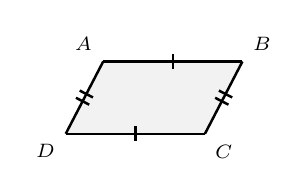
\begin{tikzpicture}[scale=0.68, every node/.style={font=\scriptsize}]
    \coordinate (D) at (0,0); \coordinate (C) at (2.6,0);
    \coordinate (A) at (0.7,1.35); \coordinate (B) at (3.3,1.35);
    \fill[gray!10] (A)--(B)--(C)--(D)--cycle;
    \draw[line width=0.9pt, tk1] (A)--(B); \draw[line width=0.9pt, tk1] (D)--(C);
    \draw[line width=0.9pt, tk2] (D)--(A); \draw[line width=0.9pt, tk2] (C)--(B);
    \node[above left=0.5pt] at (A) {$A$}; \node[above right=0.5pt] at (B) {$B$};
    \node[below right=0.5pt] at (C) {$C$}; \node[below left=0.5pt] at (D) {$D$};
  \end{tikzpicture}\par
  \chk\ គ្រប់គ្រាន់ \hspace{0.25cm} \chk\ មិនគ្រប់គ្រាន់
  &
  \vspace{2pt}
  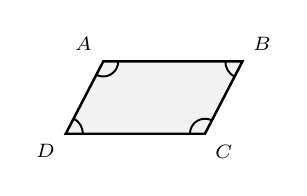
\begin{tikzpicture}[scale=0.68, every node/.style={font=\scriptsize}]
    \coordinate (D) at (0,0); \coordinate (C) at (2.6,0);
    \coordinate (A) at (0.7,1.35); \coordinate (B) at (3.3,1.35);
    \fill[gray!10] (A)--(B)--(C)--(D)--cycle;
    \draw[line width=0.9pt] (A)--(B)--(C)--(D)--cycle;
    \draw[line width=0.7pt] ($(D)+(0:0.32)$) arc (0:62:0.32);
    \draw[line width=0.7pt] ($(B)+(180:0.32)$) arc (180:242:0.32);
    \draw[line width=0.7pt] ($(A)+(-118:0.28)$) arc (-118:0:0.28);
    \draw[line width=0.7pt] ($(C)+(62:0.28)$) arc (62:180:0.28);
    \node[above left=0.5pt] at (A) {$A$}; \node[above right=0.5pt] at (B) {$B$};
    \node[below right=0.5pt] at (C) {$C$}; \node[below left=0.5pt] at (D) {$D$};
  \end{tikzpicture}\par
  \chk\ គ្រប់គ្រាន់ \hspace{0.25cm} \chk\ មិនគ្រប់គ្រាន់
  &
  \vspace{2pt}
  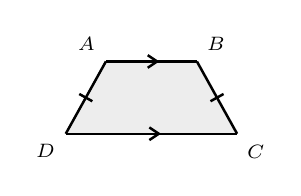
\begin{tikzpicture}[scale=0.68, every node/.style={font=\scriptsize}]
    \coordinate (D) at (0,0); \coordinate (C) at (3.2,0);
    \coordinate (A) at (0.75,1.35); \coordinate (B) at (2.45,1.35);
    \fill[gray!14] (A)--(B)--(C)--(D)--cycle;
    \draw[line width=0.9pt, par1] (A)--(B); \draw[line width=0.9pt, par1] (D)--(C);
    \draw[line width=0.9pt, tk1] (D)--(A); \draw[line width=0.9pt, tk1] (C)--(B);
    \node[above left=0.5pt] at (A) {$A$}; \node[above right=0.5pt] at (B) {$B$};
    \node[below right=0.5pt] at (C) {$C$}; \node[below left=0.5pt] at (D) {$D$};
  \end{tikzpicture}\par
  \chk\ គ្រប់គ្រាន់ \hspace{0.15cm} \chk\ មិនគ្រប់គ្រាន់ (\dotline{1.4cm}) \\
  \hline
  \rowcolor{subgray}\textbf{ករណី ឃ៖ $AB\parallel DC$ និង $AB=DC$} &
  \textbf{ករណី ង៖ $OA=OC$ និង $OB=OD$} &
  \textbf{ករណី ច៖ $AC=BD$ ប៉ុណ្ណោះ} \\
  \hline
  \vspace{2pt}
  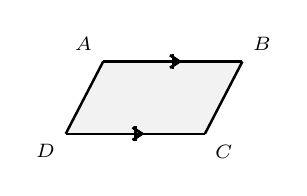
\begin{tikzpicture}[scale=0.68, every node/.style={font=\scriptsize}]
    \coordinate (D) at (0,0); \coordinate (C) at (2.6,0);
    \coordinate (A) at (0.7,1.35); \coordinate (B) at (3.3,1.35);
    \fill[gray!10] (A)--(B)--(C)--(D)--cycle;
    \draw[line width=0.9pt, par1, tk1] (A)--(B); \draw[line width=0.9pt, par1, tk1] (D)--(C);
    \draw[line width=0.9pt] (D)--(A) (C)--(B);
    \node[above left=0.5pt] at (A) {$A$}; \node[above right=0.5pt] at (B) {$B$};
    \node[below right=0.5pt] at (C) {$C$}; \node[below left=0.5pt] at (D) {$D$};
  \end{tikzpicture}\par
  \chk\ គ្រប់គ្រាន់ \hspace{0.25cm} \chk\ មិនគ្រប់គ្រាន់
  &
  \vspace{2pt}
  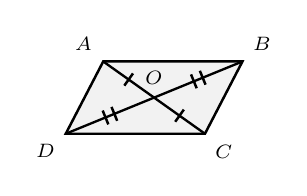
\begin{tikzpicture}[scale=0.68, every node/.style={font=\scriptsize}]
    \coordinate (D) at (0,0); \coordinate (C) at (2.6,0);
    \coordinate (A) at (0.7,1.35); \coordinate (B) at (3.3,1.35);
    \coordinate (O) at ($(A)!0.5!(C)$);
    \fill[gray!10] (A)--(B)--(C)--(D)--cycle;
    \draw[line width=0.9pt] (A)--(B)--(C)--(D)--cycle;
    \draw[line width=0.85pt, tk1] (A)--(O); \draw[line width=0.85pt, tk1] (O)--(C);
    \draw[line width=0.85pt, tk2] (B)--(O); \draw[line width=0.85pt, tk2] (O)--(D);
    \node[above=1pt] at (O) {$O$};
    \node[above left=0.5pt] at (A) {$A$}; \node[above right=0.5pt] at (B) {$B$};
    \node[below right=0.5pt] at (C) {$C$}; \node[below left=0.5pt] at (D) {$D$};
  \end{tikzpicture}\par
  \chk\ គ្រប់គ្រាន់ \hspace{0.25cm} \chk\ មិនគ្រប់គ្រាន់
  &
  \vspace{2pt}
  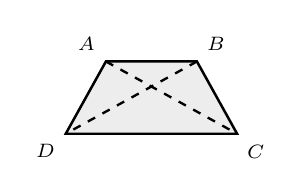
\begin{tikzpicture}[scale=0.68, every node/.style={font=\scriptsize}]
    \coordinate (D) at (0,0); \coordinate (C) at (3.2,0);
    \coordinate (A) at (0.75,1.35); \coordinate (B) at (2.45,1.35);
    \fill[gray!14] (A)--(B)--(C)--(D)--cycle;
    \draw[line width=0.9pt] (A)--(B)--(C)--(D)--cycle;
    \draw[line width=0.85pt, dashed] (A)--(C) (B)--(D);
    \node[above left=0.5pt] at (A) {$A$}; \node[above right=0.5pt] at (B) {$B$};
    \node[below right=0.5pt] at (C) {$C$}; \node[below left=0.5pt] at (D) {$D$};
  \end{tikzpicture}\par
  \chk\ គ្រប់គ្រាន់ \hspace{0.15cm} \chk\ មិនគ្រប់គ្រាន់ (\dotline{1.4cm}) \\
  \hline
\end{tabular}}

\vspace{4pt}
\textbf{សកម្មភាពទី២ — តារាងសម្រាយបញ្ជាក់បន្ថយជំនួយ (៥.៥ នាទី)៖} គូសសញ្ញា \textbf{[tracing]} លើរូប រួចបំពេញចន្លោះ៖\par\vspace{2pt}
{\renewcommand{\arraystretch}{1.20}
\begin{tabular}{|L{9.15cm}|L{9.15cm}|}
  \hline
  \rowcolor{subgray}\textbf{ផ្នែក ក៖ ទ្រឹស្ដីបទទី៦ ($AB\parallel DC$ និង $AB=DC$)} & \textbf{ផ្នែក ខ៖ ទ្រឹស្ដីបទទី៧ ($OA=OC$ និង $OB=OD$)} \\
  \hline
  \begin{center}
  \vspace{-2pt}
  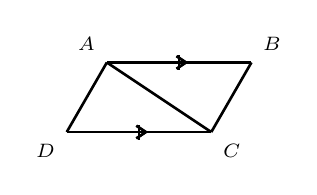
\begin{tikzpicture}[scale=0.68, every node/.style={font=\scriptsize}]
    \coordinate (D) at (0,0); \coordinate (C) at (2.7,0);
    \coordinate (A) at (0.75,1.30); \coordinate (B) at (3.45,1.30);
    \draw[line width=0.95pt, par1, tk1] (A)--(B); \draw[line width=0.95pt, par1, tk1] (D)--(C);
    \draw[line width=0.95pt] (D)--(A) (C)--(B) (A)--(C);
    \node[above left=1pt] at (A) {$A$}; \node[above right=1pt] at (B) {$B$};
    \node[below right=1pt] at (C) {$C$}; \node[below left=1pt] at (D) {$D$};
  \end{tikzpicture}
  \vspace{-3pt}
  \end{center}
  គូសអង្កត់ទ្រូង $AC$ ។ ក្នុង $\tri{ADC}$ និង $\tri{CBA}$ មាន៖\par
  ១. $DC = \dotline{1.1cm}$ (សម្មតិកម្ម)\par
  ២. $\ang{ACD} = \ang{\dotline{1.1cm}}$ (មុំឆ្លាស់ក្នុងនៃ $AB\parallel DC$)\par
  ៣. $AC$ ជាជ្រុង \dotline{1.5cm} $\Rightarrow \tri{ADC}\cg\tri{CBA}$ (\dotline{1.2cm})\par
  $\bullet$ វិបាក៖ $\ang{DAC} = \ang{\dotline{1.1cm}}$ (ឆ្លាស់ក្នុង) $\Rightarrow AD \parallel \dotline{1.0cm}$\par
  $\bullet$ ដោយ $AB\parallel DC$ និង $AD\parallel BC$ នោះ $ABCD$ ជា \dotline{2.1cm} ។
  &
  \begin{center}
  \vspace{-2pt}
  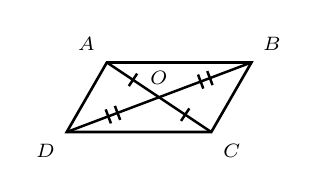
\begin{tikzpicture}[scale=0.68, every node/.style={font=\scriptsize}]
    \coordinate (D) at (0,0); \coordinate (C) at (2.7,0);
    \coordinate (A) at (0.75,1.30); \coordinate (B) at (3.45,1.30);
    \coordinate (O) at ($(A)!0.5!(C)$);
    \draw[line width=0.95pt] (A)--(B)--(C)--(D)--cycle;
    \draw[line width=0.9pt, tk1] (A)--(O); \draw[line width=0.9pt, tk1] (O)--(C);
    \draw[line width=0.9pt, tk2] (B)--(O); \draw[line width=0.9pt, tk2] (O)--(D);
    \node[above=1pt] at (O) {$O$};
    \node[above left=1pt] at (A) {$A$}; \node[above right=1pt] at (B) {$B$};
    \node[below right=1pt] at (C) {$C$}; \node[below left=1pt] at (D) {$D$};
  \end{tikzpicture}
  \vspace{-3pt}
  \end{center}
  ក្នុង $\tri{AOB}$ និង $\tri{COD}$ មាន៖\par
  ១. $OA = \dotline{1.1cm}$ ($O$ ជាចំណុចកណ្ដាលនៃ $AC$)\par
  ២. $\ang{AOB} = \ang{\dotline{1.1cm}}$ (មុំទល់កំពូល)\par
  ៣. $OB = \dotline{1.1cm}$ $\Rightarrow \tri{AOB}\cg\tri{COD}$ (\dotline{1.2cm})\par
  $\bullet$ វិបាក៖ $AB = \dotline{1.0cm}$ និង $\ang{OAB}=\ang{OCD} \Rightarrow AB \parallel \dotline{1.0cm}$\par
  $\bullet$ តាមទ្រឹស្ដីបទទី៦ នោះ $ABCD$ ជា \dotline{2.3cm} ។ \\
  \hline
\end{tabular}}

\newpage

% ============================================================================
% ទំព័រទី២៖ E3 ធនាគារហេតុផល ①–⑤ + E4 លំហាត់គំរូ ២ + E5 ប្រតិបត្តិ & Exit Check + កិច្ចការផ្ទះ
% ============================================================================
\secbar{ផ្នែកទី៣ ៖ ធនាគារហេតុផលសម្គាល់ប្រលេឡូក្រាម \cnum{1}--\cnum{5} \enbf{(E3 -- Explain)}}{៦ នាទី}
\begin{tcolorbox}[enhanced, sharp corners, colback=white, colframe=black, boxrule=0.8pt, top=3.5pt, bottom=3.5pt, left=6pt, right=6pt]
  ចតុកោណ $ABCD$ មួយជា\textbf{ប្រលេឡូក្រាម} កាលណាវាផ្ទៀងផ្ទាត់លក្ខខណ្ឌ\textbf{ណាមួយ}ក្នុងចំណោមផ្លូវទាំង ៥ ខាងក្រោម៖\par\vspace{2pt}
  \cnum{1} \textbf{និយមន័យ៖} មានជ្រុងឈម \dotline{2.3cm} ពីរៗ ($AB\parallel DC$ និង $AD\parallel BC$) ។\par\vspace{1.5pt}
  \cnum{2} \textbf{ទ្រឹស្ដីបទទី៤៖} មានជ្រុងឈម \dotline{2.3cm} ពីរៗ ($AB=DC$ និង $AD=BC$) ។\par\vspace{1.5pt}
  \cnum{3} \textbf{ទ្រឹស្ដីបទទី៥៖} មានមុំឈម \dotline{2.3cm} ពីរៗ ($\ang{A}=\ang{C}$ និង $\ang{B}=\ang{D}$) ។\par\vspace{1.5pt}
  \cnum{4} \textbf{ទ្រឹស្ដីបទទី៦៖} មាន\textbf{គូជ្រុងឈមតែមួយ} \dotline{2.2cm} ផង និង \dotline{2.2cm} ផង ($AB\parallel DC$ និង $AB=DC$) ។\par\vspace{1.5pt}
  \cnum{5} \textbf{ទ្រឹស្ដីបទទី៧៖} មានអង្កត់ទ្រូងទាំងពីរប្រសព្វគ្នាត្រង់ \dotline{2.8cm} នីមួយៗ ($OA=OC$ និង $OB=OD$) ។
\end{tcolorbox}

% --- E4 Elaborate ---
\secbar{ផ្នែកទី៤ ៖ លំហាត់គំរូអនុវត្ត \enbf{[tracing]} និងធនាគារហេតុផល \cnum{1}--\cnum{5} \enbf{(E4 -- Elaborate)}}{១០ នាទី}
{\renewcommand{\arraystretch}{1.22}
\begin{tabular}{|L{9.15cm}|L{9.15cm}|}
  \hline
  \rowcolor{subgray}\textbf{គំរូទី១ (ទំ.១៧៣--១៧៤ — ប្រលេឡូក្រាមពីរតភ្ជាប់តាម $EF$)} & \textbf{គំរូទី២ (លំហាត់ទី៣ ក ទំ.១៨៥ — ពិនិត្យចតុកោណ $EFIH$)} \\
  \hline
  គេមានចតុកោណ $ABEF$ និង $EFDC$ ជាប្រលេឡូក្រាម ។ បង្ហាញថាចតុកោណ $ABCD$ ជាប្រលេឡូក្រាម ។\par
  \begin{center}
  \vspace{-2pt}
  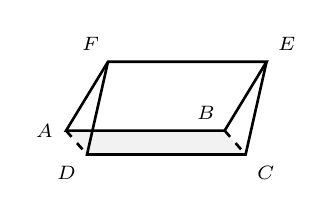
\begin{tikzpicture}[scale=0.76, every node/.style={font=\scriptsize}]
    \coordinate (D) at (0.35,0); \coordinate (C) at (3.00,0);
    \coordinate (A) at (0,0.40); \coordinate (B) at (2.65,0.40);
    \coordinate (F) at (0.70,1.55); \coordinate (E) at (3.35,1.55);
    \fill[gray!10] (A)--(B)--(C)--(D)--cycle;
    \draw[line width=0.95pt] (F)--(E)--(B)--(A)--cycle;
    \draw[line width=0.95pt] (F)--(D)--(C)--(E);
    \draw[line width=0.95pt, dashed] (A)--(D) (B)--(C);
    \node[left=1pt] at (A) {$A$}; \node[above left=0.5pt] at (B) {$B$};
    \node[below right=1pt] at (C) {$C$}; \node[below left=1pt] at (D) {$D$};
    \node[above left=1pt] at (F) {$F$}; \node[above right=1pt] at (E) {$E$};
  \end{tikzpicture}
  \vspace{-2pt}
  \end{center}
  $\bullet$ ដោយ $ABEF$ ជាប្រលេឡូក្រាម៖ $AB \parallel \dotline{0.9cm}$ និង $AB = \dotline{0.9cm}$ (១)\par
  $\bullet$ ដោយ $EFDC$ ជាប្រលេឡូក្រាម៖ $FE \parallel \dotline{0.9cm}$ និង $FE = \dotline{0.9cm}$ (២)\par
  $\bullet$ តាម (១) និង (២) គេទាញបាន៖ $AB \parallel \dotline{0.9cm}$ និង $AB = \dotline{0.9cm}$\par
  $\bullet$ ដូច្នេះ តាមហេតុផលលេខ \dotline{0.8cm} ចតុកោណ $ABCD$ ជា \dotline{2.0cm} ។
  &
  ក្នុងចតុកោណ $EFGH$ ($I \in HG$) គេឱ្យ $EH = IF$ និង $\ang{EHI} = \ang{FIG}$ ។ បង្ហាញថា $EFIH$ ជាប្រលេឡូក្រាម ។\par
  \begin{center}
  \vspace{-2pt}
  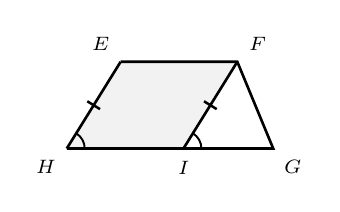
\begin{tikzpicture}[scale=0.76, every node/.style={font=\scriptsize}]
    \coordinate (H) at (0,0); \coordinate (I) at (1.95,0); \coordinate (G) at (3.45,0);
    \coordinate (E) at (0.90,1.45); \coordinate (F) at (2.85,1.45);
    \fill[gray!10] (E)--(F)--(I)--(H)--cycle;
    \draw[line width=0.95pt, tk1] (H)--(E); \draw[line width=0.95pt, tk1] (I)--(F);
    \draw[line width=0.95pt] (E)--(F)--(G)--(H);
    \draw[line width=0.7pt] ($(H)+(0:0.30)$) arc (0:58:0.30);
    \draw[line width=0.7pt] ($(I)+(0:0.30)$) arc (0:58:0.30);
    \node[below left=1pt] at (H) {$H$}; \node[below=1pt] at (I) {$I$}; \node[below right=1pt] at (G) {$G$};
    \node[above left=1pt] at (E) {$E$}; \node[above right=1pt] at (F) {$F$};
  \end{tikzpicture}
  \vspace{-2pt}
  \end{center}
  $\bullet$ ដោយ $\ang{EHI} = \ang{FIG}$ ស្ថិតនៅទីតាំងមុំ \dotline{2.2cm}\par
  ធៀបនឹងបន្ទាត់កាត់ $HG$ នោះគេបានបន្ទាត់ $EH \parallel \dotline{1.0cm}$ ។\par
  $\bullet$ រួមជាមួយសម្មតិកម្ម $EH = \dotline{1.0cm}$ (គូជ្រុងឈមតែមួយ)\par
  តាមហេតុផលលេខ \dotline{0.8cm} គេបាន $EFIH$ ជា \dotline{2.2cm} ។ \\
  \hline
\end{tabular}}

% --- E5 Evaluate ---
\secbar{ផ្នែកទី៥ ៖ លំហាត់ប្រតិបត្តិ ផ្ទៀងផ្ទាត់ជាដៃគូ និង \enbf{Exit Check (E5 -- Evaluate)}}{១០ នាទី}
\textbf{ក. លំហាត់ប្រតិបត្តិ (ទំព័រ ១៧៤)៖} គេមានត្រីកោណ $ABC$ មួយ ។ $O$ ជាចំណុចកណ្ដាលនៃ $BC$ ហើយ $D$ ជាចំណុចឆ្លុះនៃ $A$ ធៀបនឹង $O$ ។ រកប្រភេទនៃចតុកោណ $ABDC$ រួចបញ្ជាក់ហេតុផល ។\par\vspace{3pt}
\begin{tabular}{@{}L{13.15cm} C{5.65cm}@{}}
  ១. ដោយ $O$ ជាចំណុចកណ្ដាលនៃ $BC$ គេបាន៖ $OB = \dotline{2.8cm}$\par\vspace{4pt}
  ២. ដោយ $D$ ឆ្លុះនឹង $A$ ធៀបនឹង $O$ គេបាន៖ $OA = \dotline{2.8cm}$\par\vspace{4pt}
  ៣. តាមហេតុផលលេខ \dotline{0.9cm} ចតុកោណ $ABDC$ ជា \dotline{4.2cm}\par\vspace{4pt}
  ៤. \textbf{បិទបញ្ហាស៊ុមទ្វារដែក E1៖} មេជាង ខ ត្រឹមត្រូវ! ត្រូវកែឱ្យ \dotline{4.5cm}
  &
  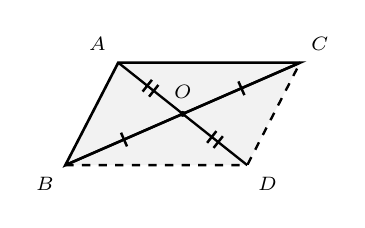
\begin{tikzpicture}[scale=0.84, baseline={(0,1.45)}, every node/.style={font=\scriptsize}]
    \coordinate (B) at (0,0); \coordinate (D) at (2.75,0);
    \coordinate (A) at (0.80,1.55); \coordinate (C) at (3.55,1.55);
    \coordinate (O) at ($(B)!0.5!(C)$);
    \fill[gray!10] (A)--(B)--(D)--(C)--cycle;
    \draw[line width=0.95pt] (A)--(B)--(C)--cycle;
    \draw[line width=0.85pt, dashed] (B)--(D)--(C);
    \draw[line width=0.85pt, tk1] (B)--(O); \draw[line width=0.85pt, tk1] (O)--(C);
    \draw[line width=0.85pt, tk2] (A)--(O); \draw[line width=0.85pt, tk2] (O)--(D);
    \fill (O) circle (1.3pt) node[above=2pt] {$O$};
    \node[above left=1pt] at (A) {$A$}; \node[below left=1pt] at (B) {$B$};
    \node[above right=1pt] at (C) {$C$}; \node[below right=1pt] at (D) {$D$};
  \end{tikzpicture}
\end{tabular}

\vspace{4pt}
\begin{tcolorbox}[enhanced, sharp corners, colback=panelgray, colframe=black, boxrule=0.8pt, top=4pt, bottom=4pt, left=6pt, right=6pt]
  \textbf{ខ. សំណួរត្រួតពិនិត្យរហ័ស (\en{Exit Check} — គូសរង្វង់ចម្លើយត្រឹមត្រូវតែ ១)៖}\par
  ក្នុងចតុកោណ $ABCD$ (ដែលមានអង្កត់ទ្រូងកាត់គ្នាត្រង់ $O$) តើលក្ខខណ្ឌណាមួយដែល \textbf{មិនគ្រប់គ្រាន់} ដើម្បីសន្និដ្ឋានថាវាជាប្រលេឡូក្រាម?\par\vspace{2pt}
  \hspace*{0.2cm}\textbf{A.} $AB=DC, AD=BC$ \hspace{0.8cm} \textbf{B.} $AB\parallel DC, AB=DC$ \hspace{0.8cm} \textbf{C.} $AB\parallel DC, AD=BC$ \hspace{0.8cm} \textbf{D.} $OA=OC, OB=OD$
\end{tcolorbox}

% --- Step 5 Homework ---
\secbar{ផ្នែកទី៦ ៖ កិច្ចការផ្ទះ និងបណ្ដាំផ្ញើ \enbf{(}សៀវភៅគោល ទំព័រ ១៨៥\enbf{)}}{ធ្វើក្នុងសៀវភៅកិច្ចការផ្ទះ}
$\bullet$ \textbf{លំហាត់ទី១ (លំហាត់ទី៣ ខ ទំព័រ ១៨៥)៖} ក្នុងចតុកោណ $EFGH$ ($I \in HG$) គេឱ្យ $EH \parallel FI$, $EH = IF$ និង $FG = IF$ ។ បង្ហាញថាចតុកោណ $EFIH$ ជាប្រលេឡូក្រាម និងប្រាប់ប្រភេទនៃត្រីកោណ $FIG$ ។\par\vspace{2pt}
$\bullet$ \textbf{លំហាត់ទី២ (លំហាត់ទី៦ ខ និងទី៧ ទំព័រ ១៨៥)៖} សង់ប្រលេឡូក្រាម $ABCD$ ដោយស្គាល់ $AD=4\unit{cm}, AB=2.5\unit{cm}, BD=3.5\unit{cm}$ ហើយប្រើ $OA'=OC', OB'=OD'$ បង្ហាញថា $A'B'C'D'$ ជាប្រលេឡូក្រាម រួចអានជាមុន \textbf{២.២ លក្ខណៈចតុកោណកែង} (ទំ.១៧៤--១៧៦) ។

\end{document}
